\documentclass[a4paper,hidelinks,14pt]{extarticle}

\usepackage[utf8]{inputenc}
\usepackage[T2A]{fontenc}
\usepackage[english, russian]{babel}
\usepackage{lipsum}
\usepackage{amsmath}
\usepackage{amssymb}
\usepackage{amsfonts}
\usepackage{mathtools}
\usepackage{datetime}
\usepackage[pdftex]{graphicx}
\usepackage{indentfirst}
\usepackage{asymptote}
\usepackage{systeme}
\usepackage[dvipsnames]{xcolor}
\usepackage{lastpage}
\usepackage{fancybox,fancyhdr}
\usepackage{hyperref}
\usepackage[framed,autolinebreaks,useliterate,numbered]{mcode}
\usepackage[font={small,it}]{caption}
\fancyhead[L]{Лабораторная работа №3}
\fancyhead[C]{}
\fancyhead[R]{Жёсткая фильтрация}
\fancyfoot[L]{}
\fancyfoot[C]{Страница \thepage\space из \pageref{LastPage}}
\fancyfoot[R]{}
\pagestyle{fancy}
\newcommand{\gt}{\textgreater}
\newcommand{\lt}{\textless}

\begin{document}
	\begin{titlepage}
		\setlength{\parindent}{0ex}
		
		\begin{center}
			\textsc{
				\vspace{1ex}
				Научно исследовательский университет ИТМО \\
				\vspace{0.5ex}
				Факультет систем управления и робототехники \\
				\vspace{0.5ex}
			}
		\end{center}
		
		\vspace{50mm}
		
		\begin{center}
			Отчет по лабораторной работе №3 \\
			Жёсткая фильтрация
		\end{center}
		
		\vspace{50mm}
		
		\begin{minipage}{.55\linewidth}
			Выполнил студент группы R3280
			
			Преподаватели
		\end{minipage}
		\hfill
		\begin{minipage}{.5\linewidth}
			\begin{flushright}
				Мовчан И. Е.
				\\
				Пашенко А.В., Перегудин А. А.
			\end{flushright}
		\end{minipage}
		
		\vfill
		\begin{center}
			Санкт-Петербург
			\\
			2024
		\end{center}
		
	\end{titlepage}
	
	\section{Жёсткие фильтры}
	
	Перед выполнением зададимся числами $a = 1$, $t_1=-10$, $t_2=5$ (отметим, что $t_1 < t_2$), составив тем самым функцию $$g(t) = \left\{ 
	\begin{array}{l}
		a,\ t \in [t_1, t_2] \\
		0,\ \text{иначе}
	\end{array} 
	\right.
	\Rightarrow
	g(t) = 
	\left\{ 
	\begin{array}{l}
		3,\ t \in [-10, 5] \\
		0,\ \text{иначе}
	\end{array} 
	\right.$$
	
	Кроме этого, выберем интервал времени T и малый шаг дискретизации dt, а также зададим массив времени t, найдя тем самым массив значений функции $g(t)$:
	\begin{lstlisting}
T = 50;
dt = 0.1;
t = -T/2:dt:T/2;
N = length(t);
g = zeros(1,N);
for i = 1:N
	if t(i) < t1 || t(i) > t2
		g(i) = 0;
	else
		g(i) = a;
	end
end
	\end{lstlisting}
	
	
	Далее зададим через константы c и d зашумлённую версию сигнала как
	\begin{lstlisting}[numbers=none]
u = g + b*(rand(size(t))-0.5) + c*sin(dt);
	\end{lstlisting}
	
	\subsection{Убираем высокие частоты}
	Положим $\text{c} = 0$, а $\text{b} = 5$, найдём Фурье-образ сигнала u, обнулим его значения для всех диапазона частот вне отрезка $[-\nu_0, \nu_0]$, где $\nu_0=5$ и сделаем обратное образование. Таким образом мы уберём маловажные шумы в сигнале, оставив только самое ценное. Результат работы представлен на рисунке \ref{1}.
	
	Параметр $b$ влияет на степень шума. $\nu_0$ на <<грубость>> его отсечения. Проверим это, используя разные параметры...
	
	\begin{figure}[h]
		\centering
		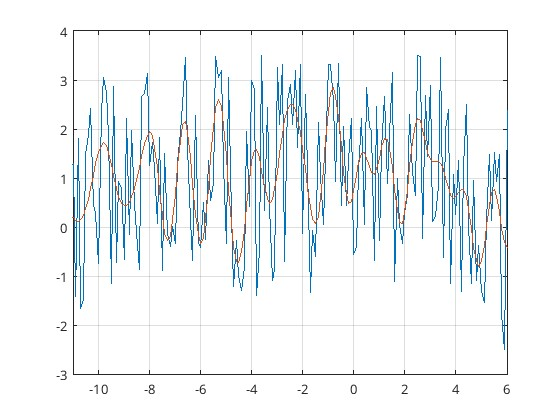
\includegraphics[scale=0.75]{./images/1.jpg}
		\caption{Зашумлённый и отфильтрованный сигналы при $b=5$, $\nu_0=5$}
		\label{1}
	\end{figure}
		
	 
	
	
	
	
\end{document}